
Avant toute chose, créer un répertoire TP09 dans votre répertoire "Informatique", "TPsup" dans votre espace personnel. Sur le site \url{https://ptsilamartin.github.io/info/TP.html}, télécharger les 3  images \texttt{vague.png}, \texttt{groupe.png} et \texttt{IRM.png} ainsi que l'animation gif \texttt{battements} que vous copiez dans votre répertoire TP09.

\begin{marginfigure}%[!h]\centering
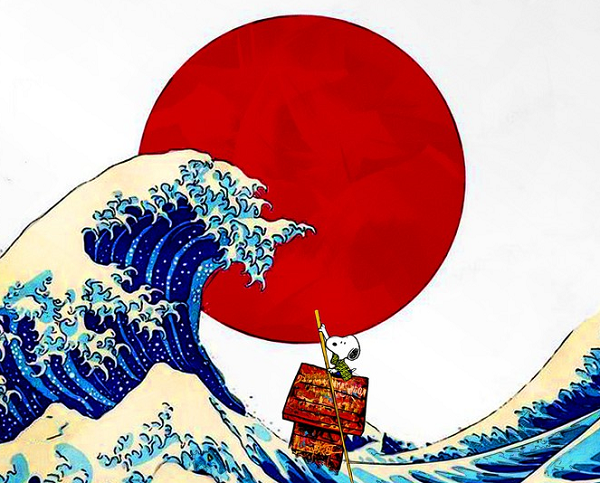
\includegraphics[width=\textwidth]{vague.png}
\end{marginfigure}

Dans ce TP, comme dans le TP08 on utilise images matricielles. Contrairement au TP08 les images sont des images colorées. La teinte de chaque pixel est codée sous la forme d'un tableau \lstinline{[R,G,B]}, \lstinline{R} codant la valeur du rouge, \lstinline{G} du vert et \lstinline{B} du bleu. \lstinline{R}, \lstinline{G}, \lstinline{B} sont des nombres réels compris entre \lstinline{0} et \lstinline{1}. 




\section*{Accentuation d'une composante de couleur}
\begin{question}
Lire l'image du fichier \texttt{vague.png} et l'afficher.
\end{question}

\begin{question}
Ecrire une fonction \texttt{accentuation} qui prend pour argument une matrice-image codée au format RGB et un flottant \texttt{ k}, et qui accentue de \texttt{k} la valeur de la composante rouge de chaque pixel. Afficher l'image obtenue avec une valeur de \texttt{ k} de~0.2. 
\end{question}




\section*{Conversion d'une image couleur en niveau de gris}

Une des possibilités pour obtenir une image en niveau de gris à partir d’une image codée sur les 3 composantes de couleur (bleu, vert, rouge) est de remplacer la valeur de chaque composante de chaque pixel par la moyenne des valeurs des 3 composantes du pixel considéré. Cette méthode est simple mais peu convaincante au niveau de l’image.

La CIE (Commission Internationale de l’Eclairage) normalise la répartition pour obtenir un niveau de gris correct. Dans sa norme 709, il est indiqué que pour les images naturelles les poids respectifs doivent être : $0.2125 * R + 0.7154 * G + 0.0721 * B.$

\textit{Rappel : pour afficher une image en niveau de gris utiliser la fonction : \texttt{plt.imshow(im, cmap="gray", vmin=0, vmax=1)}}

\begin{question}
Ecrire une fonction \texttt{niveau\_gris} qui prend pour argument une matrice-image codée au format RGB et qui convertit cette image en niveau de gris en utilisant la moyenne des composantes.
\end{question}

\begin{question} \textbf{[OPTIONNELLE : uniquement si vous êtes en avance]}
Ecrire une fonction \texttt{niveau\_gris2} qui convertit une image en niveau de gris en utilisant la norme 709.
\end{question}





\section*{Flou du visage d'une personne sur une image}


\textit{Pour des questions de protection de la vie privée, il est courant de devoir flouter les visages des personnes qui ne souhaitent pas apparaitre sur une photo. }


\subsection*{Flou avec une matrice 3x3}

\begin{question}
Lire et afficher l'image \texttt{groupe.png}.
\end{question}

\begin{question}
Créer une fonction \texttt{flou3} qui prend pour argument une image \texttt{im} et qui retourne l'image floutée en utilisant la matrice 3x3 de filtrage définie dans le cours.
\end{question}

Pour cela :
\begin{itemize}
\item déterminer : la hauteur et  la largeur de l'image ainsi que le nombre de composantes par pixel ;
\item créer une image vide ne contenant que des zéros ;
\item pour chaque pixel (hors pixels situés sur les bords de l'image), et pour chaque composante du pixel considéré :  affecter la valeur calculée à partir de la matrice de filtrage et des voisins.
\end{itemize}

\begin{question}
Tester sur l'image proposée. On obtient un effet de flou très (trop) léger.
\end{question}

\subsection*{Flou avec une matrice nxn}
Pour accentuer l'effet de flou, on propose d'utiliser une matrice de filtrage \textbf{n x n} ne contenant toujours que des 1.\\
Il faudra donc exclure du traitement une bande de pixels de largeur $b=n//2$ sur chaque bords de l'image.

\begin{question}
Créer une fonction \texttt{flou} qui prend pour argument une image \texttt{im} ainsi que la taille de l'image matrice filtre \texttt{n} et qui renvoie l'image floutée.
\end{question}

\begin{question}
Tester sur l'image proposée, pour \texttt{n=7} par exemple.
\end{question}


\subsection*{Flou sur une zone de l'image seulement}
Dans cette partie on propose de ne flouter qu'une partie de l'image, autour d'un visage par exemple. Pour cela on utilise un masque définissant la zone à traiter.

Ce masque sera une image toute noire, sauf les pixels à traiter qui seront en blanc.

\begin{question}
Créer une matrice image masque de la taille de l'image à traiter ne contenant que des pixels noirs, sauf pour les pixels situés sur les lignes allant de 80 à 179, et sur les colonnes allant de 370  à 449. Ces pixels seront blancs.
\end{question}

\textbf{Attention} : l'image masque doit avoir les mêmes caractéristiques que l'image traitée : la valeur d'un pixel blanc sera \verb![!1,1,1,1\verb!]! et celle d'un pixel noir \verb![!0,0,0,1\verb!]!, si l'image est codée sur 4 composantes (c'est le cas pour format \textbf{.png} qui gère la transparence en plus des 3 ccomposantes RGB).

A partir du masque, de l'image floutée et de l'image initiale, on peut obtenir ainsi l'image finale :

$$\text{ImageFinale}_{i,j,c} = \text{Masque}_{i,j,c} \times \text{ImageFloue}_{i,j,c}  + (1-\text{Masque}_{i,j,c}) \times \text{ImageInitiale}_{i,j,c}$$  

où $i$ et $j$ définissent la position du pixel et $c$ la composante considérée.

\begin{question}
À partir de la matrice masque, de la matrice de l'image initiale, et la matrice de l'image floutée, générer une image où seul le visage défini par le masque est flouté. L'afficher.
\end{question}

\begin{remarque}
Les images sont des tableaux \texttt{Numpy} : on pourra donc utiliser les propriétés bien pratiques des tableaux \texttt{Numpy}.\\
Il est ainsi possible de réaliser directement des opérations sur ces tableaux Numpy :  ces opéraions seront comprises comme des opérations "composantes par composantes".\\
\textbf{Exemple :} \texttt{ a=np.array([5, 2, 4]) ; b=np.array([4, 3, 6])}     \\
       Alors  : \texttt{c=a*b} donnera \texttt{array([20, 6, 24])} 

\end{remarque}


%\bigskip
\section*{Pour aller + loin : Application à une problématique d'imagerie médicale}
%\setcounter{cexo}{0}


\textit{
Les applications des algorithmes de traitement d'images sont multiples. On étudie ici l'utilisation de ces techniques pour le diagnostic et le suivi de pathologies cardio-vasculaires.}
\\
\textit{Source: Détection robuste et automatique des contours myocardiques sur des séquences IRM cardiaques marquées. Aymeric Histace, Christine Cavaro-Ménard. Les images ci-dessous proviennent toutes de cet article de recherche.}


%\noindent%

%\begin{minipage}{.6\textwidth}%
\begin{obj}
L'objectif est ici d'automatiser la détection des contours du ventricule gauche afin de pouvoir étudier la contraction pariétale.
\end{obj}

\begin{marginfigure}
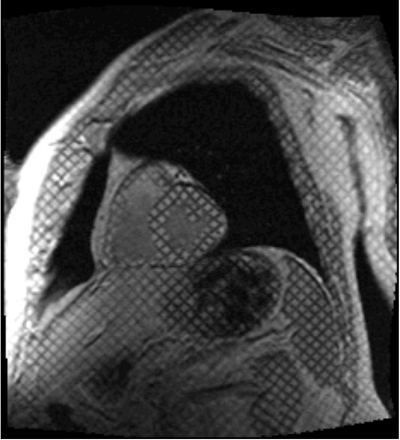
\includegraphics[width=\textwidth]{Capture5.png}
\end{marginfigure}
L'IRM cardiaque marquée permet de faire apparraitre de manière non invasive une grille (\textit{tags}) sur la zone ventriculaire gauche. Ces \textit{tags} disparaissent dans la cavité cardiaque : la cavité cardiaque est donc caractérisée par une zone homogène, la couronne mycardiqque, elle, est caractérisée par une texture en grille non homogène.

%\end{minipage}%
%\hfill
%\begin{minipage}{.35\textwidth}%
%\
%\end{minipage}


On voit ci-dessous l'image issue de l'IRM marqué (a).\\
L'image (b) est obtenue par création d'une carte de texture, dont chaque intensité de pixel s'obtient comme la somme pondérée de la moyenne (notée MOY) et de l'écart type (noté STD), d'un voisinage (de dimension T x T) autour du pixel considéré:
\begin{equation}
I(i,j)=10.MOY(i,j)-30.STD(i,j)
\end {equation}
Cette approche permet d'augmenter de manière significative le niveau de gris des pixels situés dans les zones homogènes dont l'écart type, sur le voisinage considéré, est plus faible que pour les pixels proches des \textit{tags}. Néanmoins, cette formule peut entrainer des valeurs négatives pour certains pixels : il conviendra alors de leur affecter une valeur nulle (noir).\\

Par un calcul de gradient on obtient l'image (c).\\
L'image (d) montre le contour endocardique recherché.

\begin{minipage}{1\textwidth}%
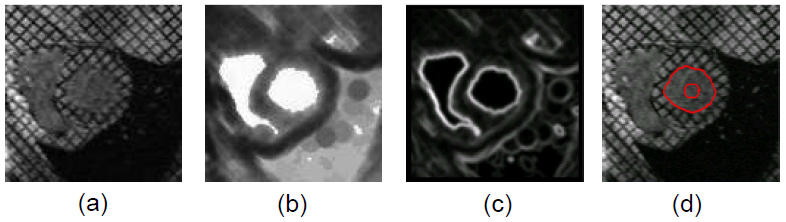
\includegraphics[width=\textwidth]{intro_IM.png}
\end{minipage}

\begin{question}
Ecrire les fonctions \texttt{Moyenne} et \texttt{EcartType} qui calculent respectivement la moyenne et l'écart type des valeurs des pixels d'une image. 
\end{question}

\begin{question}
Ecrire une fonction \texttt{CarteTexture}, qui réalise, à partir d'une image en niveau de gris, la carte de texture (b) comme expliqué ci-dessus. Tester sur l'image fournie \texttt{IRM.png} . Vous choisirez judicieusement le paramètre T le plus adapté en réalisant éventuellement plusieurs essais.   
\end{question}

\begin{question}
Déterminer le contour endocardique. Vous pourrez recadrer l'image autour de la zone souhaitée.
\end{question}





\end{document}